Many of the methods proposed in this thesis proposal are inspired by the success of many computer vision techniques. For example, in Chapter-3, we use bag-of-strokes, inspired by bag-of-words method, to represent the scene text as strokes. In Chapter-4 we take the motivations from deep learning and specifically recurrent neural networks to solve the script and language identification problem in document images at word and line level. In this chapter, Section~\ref{sec:tools} details about the Bag-of-Words (\textsc{BoW}) methods and support vector machines (\textsc{SVM}) used for script identification in the wild, Section~\ref{sec:deep} details about the deep learning and recurrent neural networks used for script and language identification in document images at word and line level.

\section{Bag-of-Words(~\textsc{BoW} and \textsc{SVM})}
\label{sec:tools}

\subsection{Image Descriptors}
In computer vision, image descriptors or visual descriptors are descriptions of the visual features of the contents in images, videos, or algorithms or applications that produce such descriptions. They describe elementary characteristics such as the shape, the color, the texture or the motion, among others. Visual descriptors are divided in two main groups:
\begin{itemize}
\item Global descriptors which are computed on whole images.
\item Local descriptors which are computed locally on a small regions or point of interests on image.
\end{itemize}

In this subsection, we will describe about common image descriptors like Local Binary Pattern (\textsc{LBP}), Scale Invariant Feature Transform (\textsc{SIFT}).

\subsubsection{Local Binary Patterns ~\textsc{LBP}}
A Local Binary Pattern (~\textsc{LBP}) ~\cite{LBPOjala2002} is a local descriptor that captures the appearance of an image in a small neighborhood around a pixel. An LBP is a string of bits, with one bit for each of the pixels in the neighborhood. Each bit is turned on or off depending on whether the intensity of the corresponding pixel is greater than the intensity of the central pixel. Figure~\ref{fig:lbpPic} depicts the basic \textsc{lbp} operator.

\begin{figure}
\centering
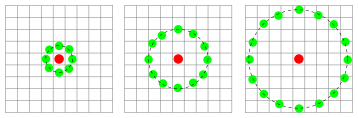
\includegraphics[scale=1]{figures/Lbp_neighbors.png}
\caption{The basic ~\textsc{lbp} operator. The figures shows the circular $(8, 1)$, $(16,2)$ and $(8,2)$ neighborhoods. The pixels are bilinearly interpolated whenever the sampling point is not at the center of a pixel. Figure source~\cite{LBPOjala2002}.}
\label{fig:lbpPic}
\end{figure}

\subsubsection{\textsc{SIFT}}
Scale-Invariant Feature Transform (\textsc{SIFT}) proposed by Lowe ~\cite{Lowe04} is one of the popular local feature detector and descriptor. SIFT descriptor is invariant to Affine transformation, Lighting changes, Noise. The original SIFT implementation includes both an interest point detector and feature descriptors at
the interest points. The descriptor associates to the regions a signature which identifies their appearance compactly and robustly. Figure 2.3 shows an example of SIFT descriptor computation at some
keypoints, and how they can be used to match points in different images. 

Computing \textsc{SIFT} descriptor at a point starts with sampling the image gradient magnitudes and orien-
tations in a region around the point. The samples are then accumulated into orientation histograms (bin
size = 8), summarizing the contents over $4 \times 4$ subregions. These orientation histograms capture the
local shape. The final descriptor is formed from a vector containing the values of $4 \times 4$ array of orientation histogram around the point. This leads to a \textsc{SIFT} feature vector with $4 \times 4 \times 8 = 128$ elements. To obtain illumination invariance, the feature vector is normalized by the square root of the sum of squared components.

\subsubsection{Gradient Based Features~\cite{Vibhor13}}
Inspired by the success of Histogram of Oriented Gradient (HOG) features~\cite{Dalal05} in many vision tasks, we adapted them to the word recognition problem. To compute the adapted HOG features, we begin by applying the Canny edge operator on the image. Note that we do not expect a clean edge map from this result. We then compute the orientation of gradient at each edge pixel. The gradient orientations are accumulated into histograms over vertical (overlapping) strips extracted from the image. The histograms are weighted by the magnitude of the gradient. An illustration of the feature computation process in shown in Fig.~\ref{fig:hogPic}. At the end of this step, we have a representation of the image in terms of a set of histograms.

\begin{figure}
\centering
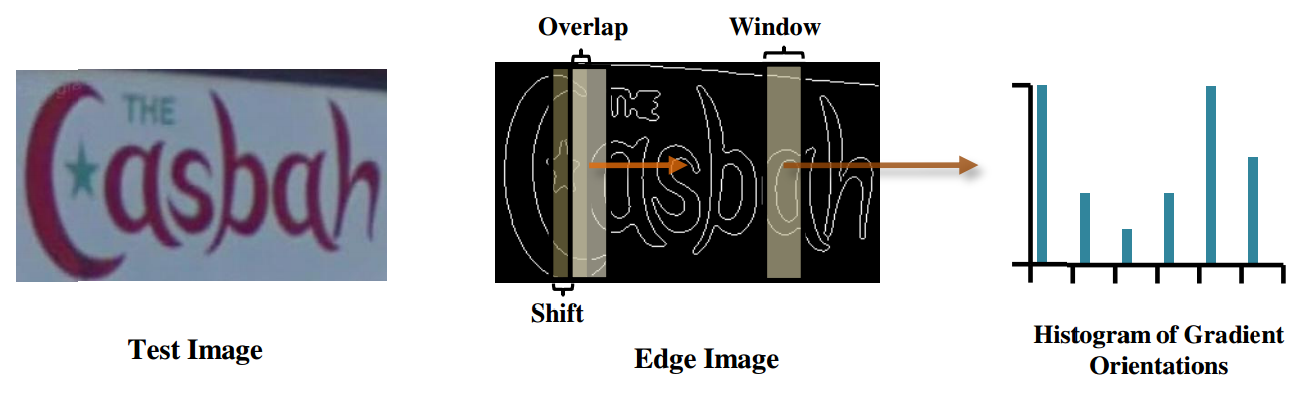
\includegraphics[scale=0.4]{figures/hogPic.png}
\caption{Histogram of Gradients computation by recording the gradient orientation at edges. Figure courtesy~\cite{Vibhor13}.}
\label{fig:hogPic}
\end{figure}

\subsection{\textit{k}-Means Clustering}
\textit{k}-means clustering is an unsupervised clustering algorithm, commonly used for constructing vo-
cabularies for Bag of Words model. Given a set of $N$ data points and number of clusters $K$, \textit{k}-means partitions the data points into K clusters, such that each data point belongs to the cluster with the nearest
mean. Figure ~\ref{fig:kmeansPic} shows an example with some data points and the clusters formed with 3 clusters.

Let the $N$ data points be $x_1, x_2, \ldots , x_n$, where $x_i \in \mathbb{R}^D$, and $K$ be the number of clusters $(K <= N)$. $S=S_1, S_2,\ldots ,S_K$ be the set of clusters each consisting of some data points, ${/mu}_i$ be the mean of points in the set $S_i$.

\begin{equation}
S = \operatornamewithlimits{argmin}_S \sum_{i=1}^{K} \sum_{x_j \in S_i} {\|{x_j - \mu_i}}\|^2
\end{equation}

The k-means algorithm uses an iterative refinement technique to solve the optimization problem.
The iterative procedure is also referred to as Lloyd’s algorithm. The algorithm starts with randomly initializing the means $\mu_1, \mu_2, \ldots, \mu_k$ . The algorithm proceeds by alternating between the following two EM steps:

\begin{itemize}
\item Expectation Step. During the assignment step, each data point is assigned to the cluster whose
mean is closest to that data point.
\begin{equation}
S_i = \left\lbrace x_p: x_p - \mu_i \leq x_p - \mu_j \| \forall 1 \leq j \leq K \right\rbrace
\end{equation}

\item Maximization Step. During the update step, the mean of each cluster is recomputed after the new assign-
ments from the previous step.
\begin{equation}
\mu_i = \frac{\sum_{x_j \in S_i} x_j}{\sum_{x_j \in S_i} 1}
\end{equation}
\end{itemize}

There is no guarantee that the algorithm will converge to the global optimum, and the result depends
on the initialisation of the cluster means. One common practice is to randomly chose K points from
the data points as the initial cluster means, and run it multiple times with different initialisations. There
are other variants of initialisations in the literature, for example \textit{k}-means++, which avoids the poor
clusterings found by the standard k-means algorithm. 

The only parameter involved in k-means clustering is K, the number of clusters. The value usually depends on the nature of data, and should be chosen appropriately by experiments.


\begin{figure}
\centering
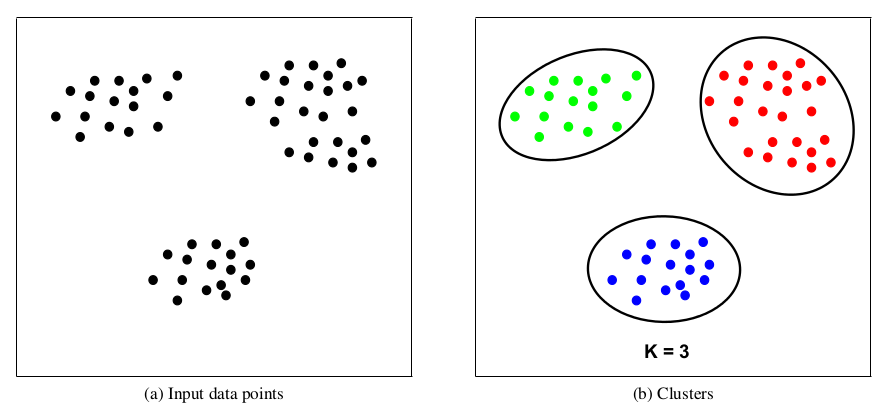
\includegraphics[scale=0.4]{figures/kmeansClust.png}
\caption{\textbf{\textit{k}-Means Clustering}. Example data points, and the clusters computed by \textit{k}-means clustering. Figure courtesy~\cite{junejaThesis}.}
\label{fig:kmeansPic}
\end{figure}

\subsection{Support Vector Machines (\textsc{SVM})}
In machine learning, classification task is a very common task. There are two types of classification tasks in machine learning:
\begin{itemize}
\item \textbf{Supervised Learning.} It is a task of inferring a function from \textit{supervised} training training data. The training data consists of training examples which are pair of an input vector and a desired output label.
\item \textbf{Unsupervised Learning.} This type of learning is used to draw inferences from the datasets consisting of input data without label information. For example, cluster analysis which is used to find the hidden patterns in data.
\end{itemize}

Support Vector Machines is a popular and powerful classification learning tool. It comes under supervised learning tasks. i.e. it learns from a given set of labelled training data and predicts  the label for an unseen test datum. We will explain SVMs for two-class case, which is also called as a ``binary'' classifier. The basic idea behind a linear classifier is to separate the given D-dimensional data points with a (D − 1) dimensional hyperplane. For a given set of points, there may exist multiple hyperplanes which can separate the data (Figure 2.6(a)). The best classifier of all these hyperplanes is the one which provides the maximum separation of the data points (Figure 2.6(b)). It essentially means that the best hyperplane should maximise the distance between the nearest points on both sides of the hyperplane (nearest points to the hyperplane from each class). This distance is defined as the ``margin'', and the SVM selects the hyperplane with the maximum margin. The hyperplane obtained is called maximum-margin hyperplane and the linear classifier is called maximum-margin classifier.

Given a set of n labelled training samples,

\begin{equation}
S =\left\lbrace \left\lbrace x_i ; y_i \right\rbrace | x_i \in D , y_i \in \left\lbrace −1, 1 \right\rbrace \right\rbrace _{i=1}^n
\end{equation}

where, $x_i$ is the $D$-dimensional data point, $y_i$ represents the class to which the $x_i$ belongs.

A separating hyperplane with w as the normal vector, can be written as
\begin{equation}
{w^T}x + b = 0
\end{equation}

Here, $b$ is called the bias term, $\frac{b}{\|w\|}$ gives the perpendicular distance from the origin to the hyperplane. Our goal is to find the $w$ and $b$, such that the ``margin'' is maximized. We can select two parallel hyperplanes which separate the data and are as far as possible (Figure 2.6). These hyperplanes can be written as follows:

\begin{equation}
{w^T}x + b = 1
{w^T}x + b = -1
\end{equation}

Now, the distance between the two parallel hyperplanes is $\frac{2}{\|w\|}$. Since the distance needs to be maximised, it translates to minimizing $\|w\|$ . Since we do not want any data points falling in between the two parallel hyperplanes, the following constraints are added:

\begin{equation}
{w^T}x_i + b \geq 1 \forall x_i s.t y_i = 1
{w^T}x_i + b \leq 1 \forall x_i s.t y_i = -1
\end{equation}

The two constraints can be combined and rewritten as:

\begin{equation}
y_i(w^{T}x_i + b) \geq 1 \forall x_i
\end{equation}

We can substitute $\|w\|$ with $\frac{1}{2}\|w\|^2$, without changing the solution, this makes the optimization problem easier to solve. The optimization problem can now be written in primal form as:

\begin{equation}
\operatornamewithlimits{min}_(w, b)\frac{1}{2} \|w\|^2 \\
subject to y_i(w^{T}x_i + b) \geq 1 \forall x_i
\end{equation}

\subsection{Implementation}

\section{Deep Learning and Recurrent Neural Networks}
\label{sec:deep}